In a variety of applications, it is necessary to localize a group of sensors or robots. In open-air environments, this can be done with GPS. In enclosed where GPS signal is not available, it is possible to do this using a variety of SLAM techniques such as bundle adjustment or pose graph optimization (PGO). These can and have been extended to optimize over a group of robots, simultaneously determining their positions~\cite{SLAM_distributed}. However, these are dependent on a complex signal processing pipeline to extract landmark or odometry measurements to optimize over. This project intends to investigate a different approach. 

The subject of this project is an implementation and extension of a novel optimization technique for distance-based relative localization. This problem is described in figure~\ref{fig:problem_desc}.
\begin{figure}[ht]
    \centering
    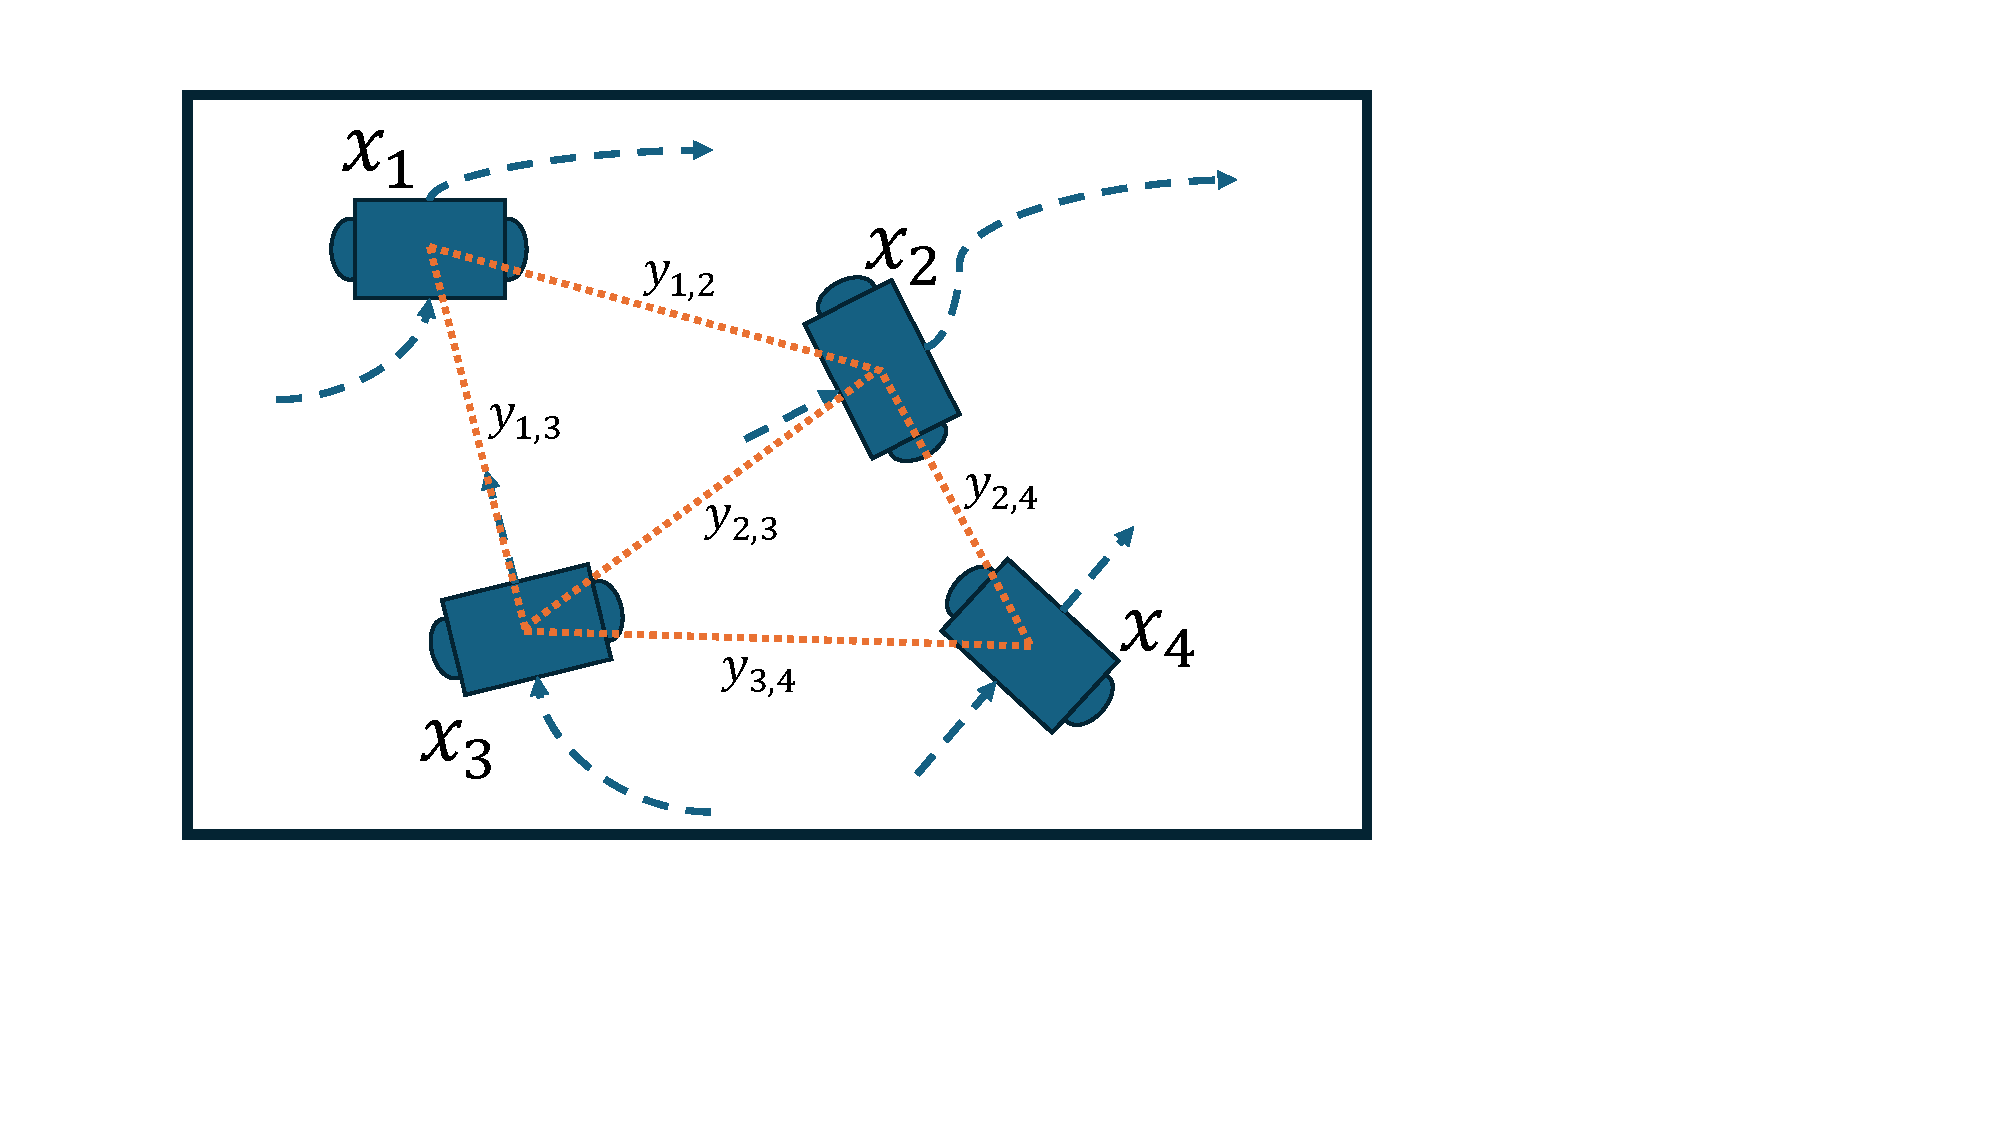
\includegraphics[width=\linewidth,trim=31mm 48mm 106mm 15mm, clip]{problem.pdf}
    \caption{Basic problem setup. In the figure, we have $N=4$ robots where $\mathbf{x}^{(i)}_t \in \mathbf{R}^3$ are the positions and angles of the robots and $y^{(i,j)}_t \in \mathbf{R}$ are the distance measurements between them.}
    \label{fig:problem_desc}
\end{figure}

SLAM  methods usually rely on measurements of external fixed points in the scene to extract measurements. This method would instead rely on the robots measuring only distance to each other. 

Some assumptions are made of the problem. It is assumed that while the distance measurements may be noisy, they are measurements of another robot in the group and not a false measurement of the environment. We will further assume additive Gaussian noise on the measurements. This project will not investigate the distributed case, and will instead assume centralized knowledge of all robot measurements. While none of the algorithms used in this project require it to be so, we have nonetheless chosen to only investigate the two-dimensional case of the problem for simplicity. 